% Created by tikzDevice version 0.12.3.1 on 2021-12-15 17:30:01
% !TEX encoding = UTF-8 Unicode
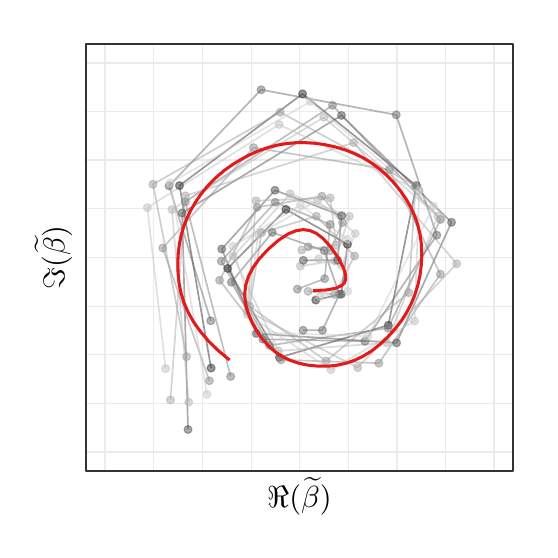
\begin{tikzpicture}[x=1pt,y=1pt]
\definecolor{fillColor}{RGB}{255,255,255}
\begin{scope}
\definecolor{drawColor}{RGB}{255,255,255}
\definecolor{fillColor}{RGB}{255,255,255}

\path[draw=drawColor,line width= 0.6pt,line join=round,line cap=round,fill=fillColor] (126.47,  0.00) rectangle (307.15,180.68);
\end{scope}
\begin{scope}
\definecolor{fillColor}{RGB}{255,255,255}

\path[fill=fillColor] (147.19, 20.71) rectangle (301.65,175.17);
\definecolor{drawColor}{gray}{0.92}

\path[draw=drawColor,line width= 0.3pt,line join=round] (147.19, 45.29) --
	(301.65, 45.29);

\path[draw=drawColor,line width= 0.3pt,line join=round] (147.19, 80.39) --
	(301.65, 80.39);

\path[draw=drawColor,line width= 0.3pt,line join=round] (147.19,115.50) --
	(301.65,115.50);

\path[draw=drawColor,line width= 0.3pt,line join=round] (147.19,150.60) --
	(301.65,150.60);

\path[draw=drawColor,line width= 0.3pt,line join=round] (171.76, 20.71) --
	(171.76,175.17);

\path[draw=drawColor,line width= 0.3pt,line join=round] (206.86, 20.71) --
	(206.86,175.17);

\path[draw=drawColor,line width= 0.3pt,line join=round] (241.97, 20.71) --
	(241.97,175.17);

\path[draw=drawColor,line width= 0.3pt,line join=round] (277.07, 20.71) --
	(277.07,175.17);

\path[draw=drawColor,line width= 0.6pt,line join=round] (147.19, 27.74) --
	(301.65, 27.74);

\path[draw=drawColor,line width= 0.6pt,line join=round] (147.19, 62.84) --
	(301.65, 62.84);

\path[draw=drawColor,line width= 0.6pt,line join=round] (147.19, 97.94) --
	(301.65, 97.94);

\path[draw=drawColor,line width= 0.6pt,line join=round] (147.19,133.05) --
	(301.65,133.05);

\path[draw=drawColor,line width= 0.6pt,line join=round] (147.19,168.15) --
	(301.65,168.15);

\path[draw=drawColor,line width= 0.6pt,line join=round] (154.21, 20.71) --
	(154.21,175.17);

\path[draw=drawColor,line width= 0.6pt,line join=round] (189.31, 20.71) --
	(189.31,175.17);

\path[draw=drawColor,line width= 0.6pt,line join=round] (224.42, 20.71) --
	(224.42,175.17);

\path[draw=drawColor,line width= 0.6pt,line join=round] (259.52, 20.71) --
	(259.52,175.17);

\path[draw=drawColor,line width= 0.6pt,line join=round] (294.63, 20.71) --
	(294.63,175.17);
\definecolor{drawColor}{RGB}{51,51,51}

\path[draw=drawColor,draw opacity=0.50,line width= 0.6pt,line join=round] (230.26, 82.56) --
	(239.47, 84.70) --
	(241.75,102.70) --
	(219.48,115.31) --
	(198.44, 93.97) --
	(217.14, 61.80) --
	(256.49, 73.46) --
	(266.60,123.90) --
	(225.50,157.07) --
	(181.03,123.92) --
	(192.43, 57.99);
\definecolor{drawColor}{RGB}{87,87,87}

\path[draw=drawColor,draw opacity=0.50,line width= 0.6pt,line join=round] (225.79, 96.89) --
	(238.17, 96.99) --
	(239.61,113.04) --
	(215.52,122.23) --
	(196.31,100.99) --
	(208.77, 70.44) --
	(259.46, 67.09) --
	(279.32,110.64) --
	(239.55,149.27) --
	(181.99,114.01) --
	(184.11, 35.79);
\definecolor{drawColor}{RGB}{110,110,110}

\path[draw=drawColor,draw opacity=0.50,line width= 0.6pt,line join=round] (225.69, 71.63) --
	(232.68, 71.64) --
	(238.80, 84.64) --
	(233.30,100.40) --
	(214.55,107.00) --
	(199.79, 89.00) --
	(211.14, 68.41) --
	(248.02, 67.64) --
	(274.00,106.00) --
	(259.34,149.48) --
	(210.53,158.55) --
	(177.27,123.82) --
	(192.32, 75.07);
\definecolor{drawColor}{RGB}{129,129,129}

\path[draw=drawColor,draw opacity=0.50,line width= 0.6pt,line join=round] (223.61, 86.49) --
	(233.50, 90.28) --
	(235.43,109.88) --
	(215.63,117.89) --
	(196.11, 96.61) --
	(213.55, 66.19) --
	(256.37, 72.40) --
	(275.38,111.72) --
	(236.33,152.90) --
	(183.15,118.11) --
	(199.52, 54.92);
\definecolor{drawColor}{RGB}{145,145,145}

\path[draw=drawColor,draw opacity=0.50,line width= 0.6pt,line join=round] (227.53,101.82) --
	(235.41,100.42) --
	(239.95,110.56) --
	(232.47,120.08) --
	(209.03,116.03) --
	(195.51, 89.70) --
	(217.71, 60.95) --
	(253.07, 59.76) --
	(275.30, 91.91) --
	(256.86,129.68) --
	(207.78,137.63) --
	(174.98,101.34) --
	(191.82, 53.40);
\definecolor{drawColor}{RGB}{159,159,159}

\path[draw=drawColor,draw opacity=0.50,line width= 0.6pt,line join=round] (227.51, 85.70) --
	(237.02, 84.55) --
	(244.25, 98.47) --
	(230.48,112.84) --
	(210.68,106.90) --
	(206.39, 80.32) --
	(234.01, 60.53) --
	(263.84, 85.23) --
	(266.36,123.84) --
	(217.42,150.44) --
	(171.46,124.40) --
	(183.58, 62.11);
\definecolor{drawColor}{RGB}{171,171,171}

\path[draw=drawColor,draw opacity=0.50,line width= 0.6pt,line join=round] (225.22,100.65) --
	(237.70,102.43) --
	(235.47,119.45) --
	(208.68,118.42) --
	(205.59, 78.59) --
	(245.43, 58.15) --
	(281.19, 95.68) --
	(243.97,139.42) --
	(183.16,120.21) --
	(177.75, 46.45);
\definecolor{drawColor}{RGB}{183,183,183}

\path[draw=drawColor,draw opacity=0.50,line width= 0.6pt,line join=round] (224.69, 94.84) --
	(237.14, 96.71) --
	(242.39,112.82) --
	(220.98,120.95) --
	(200.46, 98.36) --
	(216.81, 64.16) --
	(255.91, 67.11) --
	(274.40,112.94) --
	(233.18,148.61) --
	(178.29,115.26) --
	(184.35, 45.63);
\definecolor{drawColor}{RGB}{194,194,194}

\path[draw=drawColor,draw opacity=0.50,line width= 0.6pt,line join=round] (231.37, 97.48) --
	(239.53, 95.00) --
	(244.55,106.57) --
	(230.84,118.60) --
	(209.44,106.15) --
	(205.52, 77.33) --
	(235.75, 57.37) --
	(265.95, 74.97) --
	(267.64,122.14) --
	(217.00,145.98) --
	(169.41,115.93) --
	(176.01, 57.80);
\definecolor{drawColor}{RGB}{204,204,204}

\path[draw=drawColor,draw opacity=0.50,line width= 0.6pt,line join=round] (231.77, 83.82) --
	(241.84, 85.75) --
	(241.68,104.58) --
	(224.71,116.90) --
	(200.29,101.97) --
	(209.31, 70.88) --
	(249.14, 69.48) --
	(272.83,116.41) --
	(228.30,154.30) --
	(177.76,124.82) --
	(190.96, 48.47);
\definecolor{drawColor}{RGB}{51,51,51}
\definecolor{fillColor}{RGB}{51,51,51}

\path[draw=drawColor,draw opacity=0.50,line width= 0.4pt,line join=round,line cap=round,fill=fillColor,fill opacity=0.50] (230.26, 82.56) circle (  1.43);

\path[draw=drawColor,draw opacity=0.50,line width= 0.4pt,line join=round,line cap=round,fill=fillColor,fill opacity=0.50] (239.47, 84.70) circle (  1.43);

\path[draw=drawColor,draw opacity=0.50,line width= 0.4pt,line join=round,line cap=round,fill=fillColor,fill opacity=0.50] (241.75,102.70) circle (  1.43);

\path[draw=drawColor,draw opacity=0.50,line width= 0.4pt,line join=round,line cap=round,fill=fillColor,fill opacity=0.50] (219.48,115.31) circle (  1.43);

\path[draw=drawColor,draw opacity=0.50,line width= 0.4pt,line join=round,line cap=round,fill=fillColor,fill opacity=0.50] (198.44, 93.97) circle (  1.43);

\path[draw=drawColor,draw opacity=0.50,line width= 0.4pt,line join=round,line cap=round,fill=fillColor,fill opacity=0.50] (217.14, 61.80) circle (  1.43);

\path[draw=drawColor,draw opacity=0.50,line width= 0.4pt,line join=round,line cap=round,fill=fillColor,fill opacity=0.50] (256.49, 73.46) circle (  1.43);

\path[draw=drawColor,draw opacity=0.50,line width= 0.4pt,line join=round,line cap=round,fill=fillColor,fill opacity=0.50] (266.60,123.90) circle (  1.43);

\path[draw=drawColor,draw opacity=0.50,line width= 0.4pt,line join=round,line cap=round,fill=fillColor,fill opacity=0.50] (225.50,157.07) circle (  1.43);

\path[draw=drawColor,draw opacity=0.50,line width= 0.4pt,line join=round,line cap=round,fill=fillColor,fill opacity=0.50] (181.03,123.92) circle (  1.43);

\path[draw=drawColor,draw opacity=0.50,line width= 0.4pt,line join=round,line cap=round,fill=fillColor,fill opacity=0.50] (192.43, 57.99) circle (  1.43);
\definecolor{drawColor}{RGB}{110,110,110}
\definecolor{fillColor}{RGB}{110,110,110}

\path[draw=drawColor,draw opacity=0.50,line width= 0.4pt,line join=round,line cap=round,fill=fillColor,fill opacity=0.50] (225.69, 71.63) circle (  1.43);

\path[draw=drawColor,draw opacity=0.50,line width= 0.4pt,line join=round,line cap=round,fill=fillColor,fill opacity=0.50] (232.68, 71.64) circle (  1.43);

\path[draw=drawColor,draw opacity=0.50,line width= 0.4pt,line join=round,line cap=round,fill=fillColor,fill opacity=0.50] (238.80, 84.64) circle (  1.43);

\path[draw=drawColor,draw opacity=0.50,line width= 0.4pt,line join=round,line cap=round,fill=fillColor,fill opacity=0.50] (233.30,100.40) circle (  1.43);

\path[draw=drawColor,draw opacity=0.50,line width= 0.4pt,line join=round,line cap=round,fill=fillColor,fill opacity=0.50] (214.55,107.00) circle (  1.43);

\path[draw=drawColor,draw opacity=0.50,line width= 0.4pt,line join=round,line cap=round,fill=fillColor,fill opacity=0.50] (199.79, 89.00) circle (  1.43);

\path[draw=drawColor,draw opacity=0.50,line width= 0.4pt,line join=round,line cap=round,fill=fillColor,fill opacity=0.50] (211.14, 68.41) circle (  1.43);

\path[draw=drawColor,draw opacity=0.50,line width= 0.4pt,line join=round,line cap=round,fill=fillColor,fill opacity=0.50] (248.02, 67.64) circle (  1.43);

\path[draw=drawColor,draw opacity=0.50,line width= 0.4pt,line join=round,line cap=round,fill=fillColor,fill opacity=0.50] (274.00,106.00) circle (  1.43);

\path[draw=drawColor,draw opacity=0.50,line width= 0.4pt,line join=round,line cap=round,fill=fillColor,fill opacity=0.50] (259.34,149.48) circle (  1.43);

\path[draw=drawColor,draw opacity=0.50,line width= 0.4pt,line join=round,line cap=round,fill=fillColor,fill opacity=0.50] (210.53,158.55) circle (  1.43);

\path[draw=drawColor,draw opacity=0.50,line width= 0.4pt,line join=round,line cap=round,fill=fillColor,fill opacity=0.50] (177.27,123.82) circle (  1.43);

\path[draw=drawColor,draw opacity=0.50,line width= 0.4pt,line join=round,line cap=round,fill=fillColor,fill opacity=0.50] (192.32, 75.07) circle (  1.43);
\definecolor{drawColor}{RGB}{129,129,129}
\definecolor{fillColor}{RGB}{129,129,129}

\path[draw=drawColor,draw opacity=0.50,line width= 0.4pt,line join=round,line cap=round,fill=fillColor,fill opacity=0.50] (223.61, 86.49) circle (  1.43);

\path[draw=drawColor,draw opacity=0.50,line width= 0.4pt,line join=round,line cap=round,fill=fillColor,fill opacity=0.50] (233.50, 90.28) circle (  1.43);

\path[draw=drawColor,draw opacity=0.50,line width= 0.4pt,line join=round,line cap=round,fill=fillColor,fill opacity=0.50] (235.43,109.88) circle (  1.43);

\path[draw=drawColor,draw opacity=0.50,line width= 0.4pt,line join=round,line cap=round,fill=fillColor,fill opacity=0.50] (215.63,117.89) circle (  1.43);

\path[draw=drawColor,draw opacity=0.50,line width= 0.4pt,line join=round,line cap=round,fill=fillColor,fill opacity=0.50] (196.11, 96.61) circle (  1.43);

\path[draw=drawColor,draw opacity=0.50,line width= 0.4pt,line join=round,line cap=round,fill=fillColor,fill opacity=0.50] (213.55, 66.19) circle (  1.43);

\path[draw=drawColor,draw opacity=0.50,line width= 0.4pt,line join=round,line cap=round,fill=fillColor,fill opacity=0.50] (256.37, 72.40) circle (  1.43);

\path[draw=drawColor,draw opacity=0.50,line width= 0.4pt,line join=round,line cap=round,fill=fillColor,fill opacity=0.50] (275.38,111.72) circle (  1.43);

\path[draw=drawColor,draw opacity=0.50,line width= 0.4pt,line join=round,line cap=round,fill=fillColor,fill opacity=0.50] (236.33,152.90) circle (  1.43);

\path[draw=drawColor,draw opacity=0.50,line width= 0.4pt,line join=round,line cap=round,fill=fillColor,fill opacity=0.50] (183.15,118.11) circle (  1.43);

\path[draw=drawColor,draw opacity=0.50,line width= 0.4pt,line join=round,line cap=round,fill=fillColor,fill opacity=0.50] (199.52, 54.92) circle (  1.43);
\definecolor{drawColor}{RGB}{145,145,145}
\definecolor{fillColor}{RGB}{145,145,145}

\path[draw=drawColor,draw opacity=0.50,line width= 0.4pt,line join=round,line cap=round,fill=fillColor,fill opacity=0.50] (227.53,101.82) circle (  1.43);

\path[draw=drawColor,draw opacity=0.50,line width= 0.4pt,line join=round,line cap=round,fill=fillColor,fill opacity=0.50] (235.41,100.42) circle (  1.43);

\path[draw=drawColor,draw opacity=0.50,line width= 0.4pt,line join=round,line cap=round,fill=fillColor,fill opacity=0.50] (239.95,110.56) circle (  1.43);

\path[draw=drawColor,draw opacity=0.50,line width= 0.4pt,line join=round,line cap=round,fill=fillColor,fill opacity=0.50] (232.47,120.08) circle (  1.43);

\path[draw=drawColor,draw opacity=0.50,line width= 0.4pt,line join=round,line cap=round,fill=fillColor,fill opacity=0.50] (209.03,116.03) circle (  1.43);

\path[draw=drawColor,draw opacity=0.50,line width= 0.4pt,line join=round,line cap=round,fill=fillColor,fill opacity=0.50] (195.51, 89.70) circle (  1.43);

\path[draw=drawColor,draw opacity=0.50,line width= 0.4pt,line join=round,line cap=round,fill=fillColor,fill opacity=0.50] (217.71, 60.95) circle (  1.43);

\path[draw=drawColor,draw opacity=0.50,line width= 0.4pt,line join=round,line cap=round,fill=fillColor,fill opacity=0.50] (253.07, 59.76) circle (  1.43);

\path[draw=drawColor,draw opacity=0.50,line width= 0.4pt,line join=round,line cap=round,fill=fillColor,fill opacity=0.50] (275.30, 91.91) circle (  1.43);

\path[draw=drawColor,draw opacity=0.50,line width= 0.4pt,line join=round,line cap=round,fill=fillColor,fill opacity=0.50] (256.86,129.68) circle (  1.43);

\path[draw=drawColor,draw opacity=0.50,line width= 0.4pt,line join=round,line cap=round,fill=fillColor,fill opacity=0.50] (207.78,137.63) circle (  1.43);

\path[draw=drawColor,draw opacity=0.50,line width= 0.4pt,line join=round,line cap=round,fill=fillColor,fill opacity=0.50] (174.98,101.34) circle (  1.43);

\path[draw=drawColor,draw opacity=0.50,line width= 0.4pt,line join=round,line cap=round,fill=fillColor,fill opacity=0.50] (191.82, 53.40) circle (  1.43);
\definecolor{drawColor}{RGB}{159,159,159}
\definecolor{fillColor}{RGB}{159,159,159}

\path[draw=drawColor,draw opacity=0.50,line width= 0.4pt,line join=round,line cap=round,fill=fillColor,fill opacity=0.50] (227.51, 85.70) circle (  1.43);

\path[draw=drawColor,draw opacity=0.50,line width= 0.4pt,line join=round,line cap=round,fill=fillColor,fill opacity=0.50] (237.02, 84.55) circle (  1.43);

\path[draw=drawColor,draw opacity=0.50,line width= 0.4pt,line join=round,line cap=round,fill=fillColor,fill opacity=0.50] (244.25, 98.47) circle (  1.43);

\path[draw=drawColor,draw opacity=0.50,line width= 0.4pt,line join=round,line cap=round,fill=fillColor,fill opacity=0.50] (230.48,112.84) circle (  1.43);

\path[draw=drawColor,draw opacity=0.50,line width= 0.4pt,line join=round,line cap=round,fill=fillColor,fill opacity=0.50] (210.68,106.90) circle (  1.43);

\path[draw=drawColor,draw opacity=0.50,line width= 0.4pt,line join=round,line cap=round,fill=fillColor,fill opacity=0.50] (206.39, 80.32) circle (  1.43);

\path[draw=drawColor,draw opacity=0.50,line width= 0.4pt,line join=round,line cap=round,fill=fillColor,fill opacity=0.50] (234.01, 60.53) circle (  1.43);

\path[draw=drawColor,draw opacity=0.50,line width= 0.4pt,line join=round,line cap=round,fill=fillColor,fill opacity=0.50] (263.84, 85.23) circle (  1.43);

\path[draw=drawColor,draw opacity=0.50,line width= 0.4pt,line join=round,line cap=round,fill=fillColor,fill opacity=0.50] (266.36,123.84) circle (  1.43);

\path[draw=drawColor,draw opacity=0.50,line width= 0.4pt,line join=round,line cap=round,fill=fillColor,fill opacity=0.50] (217.42,150.44) circle (  1.43);

\path[draw=drawColor,draw opacity=0.50,line width= 0.4pt,line join=round,line cap=round,fill=fillColor,fill opacity=0.50] (171.46,124.40) circle (  1.43);

\path[draw=drawColor,draw opacity=0.50,line width= 0.4pt,line join=round,line cap=round,fill=fillColor,fill opacity=0.50] (183.58, 62.11) circle (  1.43);
\definecolor{drawColor}{RGB}{171,171,171}
\definecolor{fillColor}{RGB}{171,171,171}

\path[draw=drawColor,draw opacity=0.50,line width= 0.4pt,line join=round,line cap=round,fill=fillColor,fill opacity=0.50] (225.22,100.65) circle (  1.43);

\path[draw=drawColor,draw opacity=0.50,line width= 0.4pt,line join=round,line cap=round,fill=fillColor,fill opacity=0.50] (237.70,102.43) circle (  1.43);

\path[draw=drawColor,draw opacity=0.50,line width= 0.4pt,line join=round,line cap=round,fill=fillColor,fill opacity=0.50] (235.47,119.45) circle (  1.43);

\path[draw=drawColor,draw opacity=0.50,line width= 0.4pt,line join=round,line cap=round,fill=fillColor,fill opacity=0.50] (208.68,118.42) circle (  1.43);

\path[draw=drawColor,draw opacity=0.50,line width= 0.4pt,line join=round,line cap=round,fill=fillColor,fill opacity=0.50] (205.59, 78.59) circle (  1.43);

\path[draw=drawColor,draw opacity=0.50,line width= 0.4pt,line join=round,line cap=round,fill=fillColor,fill opacity=0.50] (245.43, 58.15) circle (  1.43);

\path[draw=drawColor,draw opacity=0.50,line width= 0.4pt,line join=round,line cap=round,fill=fillColor,fill opacity=0.50] (281.19, 95.68) circle (  1.43);

\path[draw=drawColor,draw opacity=0.50,line width= 0.4pt,line join=round,line cap=round,fill=fillColor,fill opacity=0.50] (243.97,139.42) circle (  1.43);

\path[draw=drawColor,draw opacity=0.50,line width= 0.4pt,line join=round,line cap=round,fill=fillColor,fill opacity=0.50] (183.16,120.21) circle (  1.43);

\path[draw=drawColor,draw opacity=0.50,line width= 0.4pt,line join=round,line cap=round,fill=fillColor,fill opacity=0.50] (177.75, 46.45) circle (  1.43);
\definecolor{drawColor}{RGB}{183,183,183}
\definecolor{fillColor}{RGB}{183,183,183}

\path[draw=drawColor,draw opacity=0.50,line width= 0.4pt,line join=round,line cap=round,fill=fillColor,fill opacity=0.50] (224.69, 94.84) circle (  1.43);

\path[draw=drawColor,draw opacity=0.50,line width= 0.4pt,line join=round,line cap=round,fill=fillColor,fill opacity=0.50] (237.14, 96.71) circle (  1.43);

\path[draw=drawColor,draw opacity=0.50,line width= 0.4pt,line join=round,line cap=round,fill=fillColor,fill opacity=0.50] (242.39,112.82) circle (  1.43);

\path[draw=drawColor,draw opacity=0.50,line width= 0.4pt,line join=round,line cap=round,fill=fillColor,fill opacity=0.50] (220.98,120.95) circle (  1.43);

\path[draw=drawColor,draw opacity=0.50,line width= 0.4pt,line join=round,line cap=round,fill=fillColor,fill opacity=0.50] (200.46, 98.36) circle (  1.43);

\path[draw=drawColor,draw opacity=0.50,line width= 0.4pt,line join=round,line cap=round,fill=fillColor,fill opacity=0.50] (216.81, 64.16) circle (  1.43);

\path[draw=drawColor,draw opacity=0.50,line width= 0.4pt,line join=round,line cap=round,fill=fillColor,fill opacity=0.50] (255.91, 67.11) circle (  1.43);

\path[draw=drawColor,draw opacity=0.50,line width= 0.4pt,line join=round,line cap=round,fill=fillColor,fill opacity=0.50] (274.40,112.94) circle (  1.43);

\path[draw=drawColor,draw opacity=0.50,line width= 0.4pt,line join=round,line cap=round,fill=fillColor,fill opacity=0.50] (233.18,148.61) circle (  1.43);

\path[draw=drawColor,draw opacity=0.50,line width= 0.4pt,line join=round,line cap=round,fill=fillColor,fill opacity=0.50] (178.29,115.26) circle (  1.43);

\path[draw=drawColor,draw opacity=0.50,line width= 0.4pt,line join=round,line cap=round,fill=fillColor,fill opacity=0.50] (184.35, 45.63) circle (  1.43);
\definecolor{drawColor}{RGB}{194,194,194}
\definecolor{fillColor}{RGB}{194,194,194}

\path[draw=drawColor,draw opacity=0.50,line width= 0.4pt,line join=round,line cap=round,fill=fillColor,fill opacity=0.50] (231.37, 97.48) circle (  1.43);

\path[draw=drawColor,draw opacity=0.50,line width= 0.4pt,line join=round,line cap=round,fill=fillColor,fill opacity=0.50] (239.53, 95.00) circle (  1.43);

\path[draw=drawColor,draw opacity=0.50,line width= 0.4pt,line join=round,line cap=round,fill=fillColor,fill opacity=0.50] (244.55,106.57) circle (  1.43);

\path[draw=drawColor,draw opacity=0.50,line width= 0.4pt,line join=round,line cap=round,fill=fillColor,fill opacity=0.50] (230.84,118.60) circle (  1.43);

\path[draw=drawColor,draw opacity=0.50,line width= 0.4pt,line join=round,line cap=round,fill=fillColor,fill opacity=0.50] (209.44,106.15) circle (  1.43);

\path[draw=drawColor,draw opacity=0.50,line width= 0.4pt,line join=round,line cap=round,fill=fillColor,fill opacity=0.50] (205.52, 77.33) circle (  1.43);

\path[draw=drawColor,draw opacity=0.50,line width= 0.4pt,line join=round,line cap=round,fill=fillColor,fill opacity=0.50] (235.75, 57.37) circle (  1.43);

\path[draw=drawColor,draw opacity=0.50,line width= 0.4pt,line join=round,line cap=round,fill=fillColor,fill opacity=0.50] (265.95, 74.97) circle (  1.43);

\path[draw=drawColor,draw opacity=0.50,line width= 0.4pt,line join=round,line cap=round,fill=fillColor,fill opacity=0.50] (267.64,122.14) circle (  1.43);

\path[draw=drawColor,draw opacity=0.50,line width= 0.4pt,line join=round,line cap=round,fill=fillColor,fill opacity=0.50] (217.00,145.98) circle (  1.43);

\path[draw=drawColor,draw opacity=0.50,line width= 0.4pt,line join=round,line cap=round,fill=fillColor,fill opacity=0.50] (169.41,115.93) circle (  1.43);

\path[draw=drawColor,draw opacity=0.50,line width= 0.4pt,line join=round,line cap=round,fill=fillColor,fill opacity=0.50] (176.01, 57.80) circle (  1.43);
\definecolor{drawColor}{RGB}{204,204,204}
\definecolor{fillColor}{RGB}{204,204,204}

\path[draw=drawColor,draw opacity=0.50,line width= 0.4pt,line join=round,line cap=round,fill=fillColor,fill opacity=0.50] (231.77, 83.82) circle (  1.43);

\path[draw=drawColor,draw opacity=0.50,line width= 0.4pt,line join=round,line cap=round,fill=fillColor,fill opacity=0.50] (241.84, 85.75) circle (  1.43);

\path[draw=drawColor,draw opacity=0.50,line width= 0.4pt,line join=round,line cap=round,fill=fillColor,fill opacity=0.50] (241.68,104.58) circle (  1.43);

\path[draw=drawColor,draw opacity=0.50,line width= 0.4pt,line join=round,line cap=round,fill=fillColor,fill opacity=0.50] (224.71,116.90) circle (  1.43);

\path[draw=drawColor,draw opacity=0.50,line width= 0.4pt,line join=round,line cap=round,fill=fillColor,fill opacity=0.50] (200.29,101.97) circle (  1.43);

\path[draw=drawColor,draw opacity=0.50,line width= 0.4pt,line join=round,line cap=round,fill=fillColor,fill opacity=0.50] (209.31, 70.88) circle (  1.43);

\path[draw=drawColor,draw opacity=0.50,line width= 0.4pt,line join=round,line cap=round,fill=fillColor,fill opacity=0.50] (249.14, 69.48) circle (  1.43);

\path[draw=drawColor,draw opacity=0.50,line width= 0.4pt,line join=round,line cap=round,fill=fillColor,fill opacity=0.50] (272.83,116.41) circle (  1.43);

\path[draw=drawColor,draw opacity=0.50,line width= 0.4pt,line join=round,line cap=round,fill=fillColor,fill opacity=0.50] (228.30,154.30) circle (  1.43);

\path[draw=drawColor,draw opacity=0.50,line width= 0.4pt,line join=round,line cap=round,fill=fillColor,fill opacity=0.50] (177.76,124.82) circle (  1.43);

\path[draw=drawColor,draw opacity=0.50,line width= 0.4pt,line join=round,line cap=round,fill=fillColor,fill opacity=0.50] (190.96, 48.47) circle (  1.43);
\definecolor{drawColor}{RGB}{87,87,87}
\definecolor{fillColor}{RGB}{87,87,87}

\path[draw=drawColor,draw opacity=0.50,line width= 0.4pt,line join=round,line cap=round,fill=fillColor,fill opacity=0.50] (225.79, 96.89) circle (  1.43);

\path[draw=drawColor,draw opacity=0.50,line width= 0.4pt,line join=round,line cap=round,fill=fillColor,fill opacity=0.50] (238.17, 96.99) circle (  1.43);

\path[draw=drawColor,draw opacity=0.50,line width= 0.4pt,line join=round,line cap=round,fill=fillColor,fill opacity=0.50] (239.61,113.04) circle (  1.43);

\path[draw=drawColor,draw opacity=0.50,line width= 0.4pt,line join=round,line cap=round,fill=fillColor,fill opacity=0.50] (215.52,122.23) circle (  1.43);

\path[draw=drawColor,draw opacity=0.50,line width= 0.4pt,line join=round,line cap=round,fill=fillColor,fill opacity=0.50] (196.31,100.99) circle (  1.43);

\path[draw=drawColor,draw opacity=0.50,line width= 0.4pt,line join=round,line cap=round,fill=fillColor,fill opacity=0.50] (208.77, 70.44) circle (  1.43);

\path[draw=drawColor,draw opacity=0.50,line width= 0.4pt,line join=round,line cap=round,fill=fillColor,fill opacity=0.50] (259.46, 67.09) circle (  1.43);

\path[draw=drawColor,draw opacity=0.50,line width= 0.4pt,line join=round,line cap=round,fill=fillColor,fill opacity=0.50] (279.32,110.64) circle (  1.43);

\path[draw=drawColor,draw opacity=0.50,line width= 0.4pt,line join=round,line cap=round,fill=fillColor,fill opacity=0.50] (239.55,149.27) circle (  1.43);

\path[draw=drawColor,draw opacity=0.50,line width= 0.4pt,line join=round,line cap=round,fill=fillColor,fill opacity=0.50] (181.99,114.01) circle (  1.43);

\path[draw=drawColor,draw opacity=0.50,line width= 0.4pt,line join=round,line cap=round,fill=fillColor,fill opacity=0.50] (184.11, 35.79) circle (  1.43);
\definecolor{drawColor}{RGB}{227,26,28}

\path[draw=drawColor,line width= 1.1pt,line join=round] (229.25, 85.96) --
	(234.27, 86.21) --
	(237.53, 86.85) --
	(239.50, 87.71) --
	(240.58, 88.72) --
	(241.08, 89.95) --
	(241.06, 91.65) --
	(240.29, 94.13) --
	(238.45, 97.68) --
	(235.57,101.89) --
	(232.86,104.85) --
	(230.39,106.70) --
	(228.06,107.70) --
	(225.73,108.00) --
	(223.22,107.63) --
	(220.36,106.48) --
	(216.99,104.31) --
	(213.10,100.95) --
	(209.86, 97.45) --
	(207.51, 94.17) --
	(205.92, 91.05) --
	(204.97, 88.01) --
	(204.60, 84.97) --
	(204.79, 81.84) --
	(205.57, 78.50) --
	(207.04, 74.87) --
	(208.96, 71.36) --
	(211.03, 68.40) --
	(213.24, 65.91) --
	(215.62, 63.84) --
	(218.20, 62.14) --
	(221.02, 60.77) --
	(224.14, 59.72) --
	(227.62, 59.01) --
	(231.37, 58.65) --
	(234.91, 58.68) --
	(238.26, 59.06) --
	(241.45, 59.80) --
	(244.53, 60.89) --
	(247.53, 62.35) --
	(250.50, 64.21) --
	(253.46, 66.53) --
	(256.39, 69.31) --
	(259.03, 72.24) --
	(261.30, 75.23) --
	(263.23, 78.29) --
	(264.85, 81.45) --
	(266.17, 84.73) --
	(267.21, 88.14) --
	(267.97, 91.73) --
	(268.43, 95.53) --
	(268.58, 99.33) --
	(268.41,102.92) --
	(267.93,106.36) --
	(267.15,109.66) --
	(266.06,112.85) --
	(264.66,115.98) --
	(262.92,119.05) --
	(260.81,122.10) --
	(258.38,125.06) --
	(255.83,127.71) --
	(253.16,130.05) --
	(250.36,132.12) --
	(247.42,133.92) --
	(244.30,135.47) --
	(240.99,136.78) --
	(237.45,137.85) --
	(233.69,138.68) --
	(229.98,139.21) --
	(226.40,139.44) --
	(222.92,139.40) --
	(219.52,139.08) --
	(216.19,138.49) --
	(212.88,137.62) --
	(209.60,136.46) --
	(206.31,135.00) --
	(203.13,133.32) --
	(200.20,131.51) --
	(197.49,129.59) --
	(194.99,127.53) --
	(192.68,125.34) --
	(190.54,123.00) --
	(188.56,120.50) --
	(186.75,117.83) --
	(185.10,115.01) --
	(183.72,112.13) --
	(182.58,109.18) --
	(181.68,106.14) --
	(181.02,102.99) --
	(180.60, 99.72) --
	(180.42, 96.29) --
	(180.50, 92.68) --
	(180.84, 88.90) --
	(181.55, 85.20) --
	(182.65, 81.63) --
	(184.15, 78.14) --
	(186.09, 74.70) --
	(188.50, 71.27) --
	(191.44, 67.83) --
	(194.95, 64.37) --
	(199.12, 60.87);
\definecolor{drawColor}{gray}{0.20}

\path[draw=drawColor,line width= 0.6pt,line join=round,line cap=round] (147.19, 20.71) rectangle (301.65,175.17);
\end{scope}
\begin{scope}
\definecolor{drawColor}{RGB}{0,0,0}

\node[text=drawColor,anchor=base,inner sep=0pt, outer sep=0pt, scale=  1.10] at (224.42,  7.64) {$\Re(\widetilde\beta)$};
\end{scope}
\begin{scope}
\definecolor{drawColor}{RGB}{0,0,0}

\node[text=drawColor,rotate= 90.00,anchor=base,inner sep=0pt, outer sep=0pt, scale=  1.10] at (139.55, 97.94) {$\Im(\widetilde\beta)$};
\end{scope}
\end{tikzpicture}
